\documentclass[letterpaper,10pt,titlepage]{article}

\usepackage{graphicx}
\usepackage{pdfpages}
\usepackage{amssymb}
\usepackage{amsmath}
\usepackage{amsthm}

\usepackage{alltt}
\usepackage{float}
\usepackage{color}
\usepackage{verbatim}

\usepackage{geometry}
\geometry{textheight=10in, textwidth=7.5in}

\usepackage{hyperref}

\def\name{Vlad Predovic}

%pull in the necessary preamble matter for pygments output
\input{pygments.tex}

%% The following metadata will show up in the PDF properties
\hypersetup{
  colorlinks = true,
  urlcolor = black,
  pdfauthor = {\name},
  pdfkeywords = {cs311 ``operating systems'' files filesystem I/O},
  pdftitle = {CS 311 Project 4: Threads and processes},
  pdfsubject = {CS 311 Project 4},
  pdfpagemode = UseNone
}

\parindent = 0.0 in
\parskip = 0.2 in

\begin{document}
\section{Design}


\begin{itemize} 
\item Implementations: Feed segments of the array into the thread or process depending on the quantity I am
using. For the process version I will mount my struct containing the info. I should not have to lock my processes
or threads since I am offset indexing to access the data.

\item Alot of information and examples were provided regarding the pthreads library. I plan to alter examples in class 
to fit my implementations and read up on the documentation.

\item I will mount my bitmap as part of the struct for the process version. For the threads version I will just include the bitmap inside the struct.
The bitmap will be created after the initial prime manipulation. ~In retrospect....this was a huge, painful mistake. Lesson learned.

\item I will use my sieve implementation from HW assignment one to create the bit array that will then be manipulated throughout the assignment.
\ldots 
\end{itemize}

Retrospective comments on design(self hate section):
	My initial design was to copy sections of an array into different threads or processes and have it compile the results after all processes were
	completed. Although it worked relatively well with low intervals, I quickly understood this design was flawed so I reset and started over.
	After discussing with peers and the instructor, i redesigned my system so i could initally feed my primes into a bit mask. I used chars to mask the bits,
	and I was able to fit four numbers per char as I wanted to leave a bit for designating the happy/sad state of the number. 
	My plan was to mask my bit array in a file of this format and then feed it through the threads/processes which would each be given offsets depending on the amount.
	
	This part was difficult until i implemented a global array which simplified alot of the copying I was previously doing. 
	I used primarily the examples from class and man pages to apply threads and processes. In order to handle signals I used the previous assignments work and revisited 
	the textbook.
	




\section{Challenges}
My greatest difficult dealt with memory allocation. I learned a lot having to manipulate different types in order to efficiently pass my data
along to different processes. I struggled greatly with even getting my algorithm to give me a bit array with uint entries.


\section{Answers}
\subsection{Main point of the assignment}
More programming at the system level. For me the most important port of this assignment was learning to manipulate
bits and functionality(the threads and processes) when dealing with heavy loads on memory and process time. I feel this
was a critical skill to pick up although I have not seen the sun in the last week because of it.

\subsection{Solution Accuracy}
I used a variety of primitive testing methods, primarily printing the many iterators I used to keep track of my variables.
I am confident that my solution works correctly as the list of Happy Primes for the first few numbers is not that extensive and creating a simple algorithm
to print my results showed that my answers were in line with expected results for the first few thousand numbers.

However, comparing the size of output files and variables that I used to record bit array sizes I found that the greater my range that I tested,
the larger variety I found.
My 7 different thread samples(running at 32, 25, 16....etc) produced a standard deviation of bytes of .08 percent of the total range checked.
This is alarmingly significant, an acceptable number would be around .0001 or lower. This data suggests that near the later part
of my data I have increasingly erroneous data.


Also the command xxd -b was great for checking my bit masks. It prints the contents of a file in binary to the command line.
Output example of first 3 happies for happy primes file:
0000000: 00000111 00000000 00000000 00000000 00001101 00000000  ......
0000006: 00000000 00000000 00010011 00000000 00000000 00000000 

\subsection{Learnings}
My understanding of how to manipulate memory and make programs much more efficient has increased greatly.
I feel this is a very important set of tools to keep in mind when building programs to be memory-efficient and short on run-time.

\section{Work log}
commit b4fb479ffa8c6bfe0950cdadad0368804328d2df
Author: Vladis466 <predovic900@gmail.com>
Date:   Mon Aug 3 22:05:41 2015 -0700

    Final tweaks, but getting latex file ready so pushing for logs. Signak checking updated, still working on correct use of process version. 
	I found my mistakes but ran out of time to fix them regarding hitting UINT MAX. I simply was not allocating memory on the heap on numerous occasions. Fixed alot of issues but sieve needs a rewrite and I am able to max out my threads as far as my sieve can currently go.

commit 3fc0ebed59db927783a0782fd26c27f4d59f4c56
Author: Vladis466 <predovic900@gmail.com>
Date:   Sun Aug 2 03:00:43 2015 -0700

    Having this strange issue where my parameters dont get passed into the children. Further disciplinary action required.

commit 1714a10ef1e501204cb1c84ede86894898289997
Author: Vladis466 <predovic900@gmail.com>
Date:   Sat Aug 1 21:07:12 2015 -0700

    Working on system version. My prime finder wont reach UintMax and I hate life because of it. However threaded is working well, the global bitmask array works like a charm,
	and I have succesfully extracted happiness from all primes selected

commit 9266c7565ac5d58662652c3bab5fe418d8d7bf34
Author: Vladis466 <predovic900@gmail.com>
Date:   Fri Jul 31 22:16:22 2015 -0700

    Happy primes are correctly inserted into the BIT MASK IT WORK IM NOT AN IDIOT. Still cant hit UINT max, implementing threads.

commit 557b38fad5929c1984121649def5715bba8e4797
Author: Vladis466 <predovic900@gmail.com>
Date:   Fri Jul 31 20:37:36 2015 -0700

    happy prime finder is working correctly, at least on low numbers. Checking the bit map every time is slow and painful. Next going to try to implement the threads correctly, 
	or create the output bitmask from the List array bitmap.

commit 328945fdcb5b4e6bc2602216b9294778c72099aa
Author: Vladis466 <predovic900@gmail.com>
Date:   Fri Jul 31 17:29:46 2015 -0700

    Began implementing bit map. Forgot to update lately. Having issues reaching uintmax. Not sure how to go precisely though bitmap.

commit c3e1cb751701e9b69c10a69602d50557a72c1035
Author: Vladis466 <predovic900@gmail.com>
Date:   Wed Jul 22 22:47:10 2015 -0700

    logged

\section{Results}
\begin{figure}
    \centering
    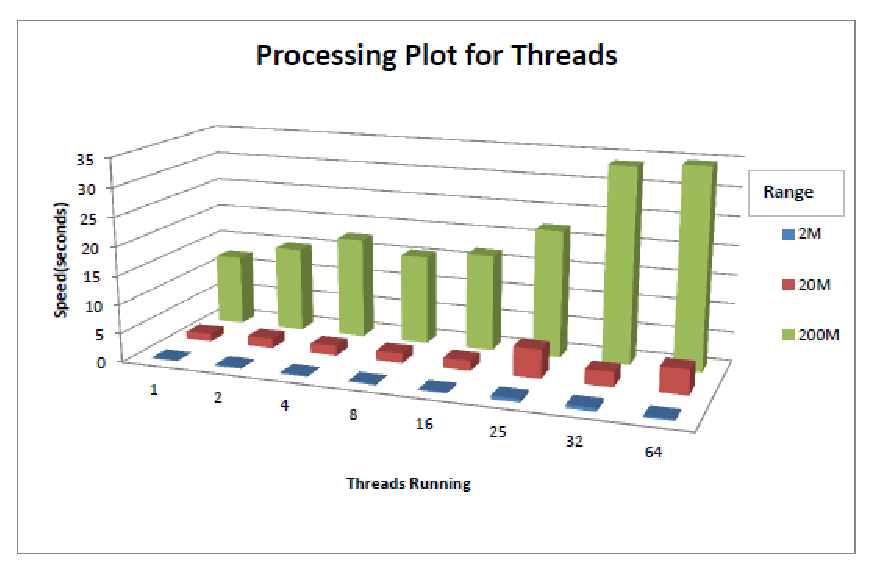
\includegraphics[width=0.8\textwidth]{graph.eps}
\end{figure}


200,000,000 with 1 threads:
intmask size:  12562336
Elapsed: 12.320000 seconds
12.178u 0.155s 0:17.12 71.9%    0+0k 0+109944io 0pf+0w

20,000,000 with 1 threads:
intmask size:  1399720
Elapsed: 1.310000 seconds
1.315u 0.010s 0:04.45 29.6%     0+0k 0+11144io 0pf+0w


2,000,000 with 1 threads:
intmask size:  166472
Elapsed: 0.150000 seconds
0.151u 0.005s 0:03.97 3.7%      0+0k 0+1160io 0pf+0w





200,000,000 with 2 threads:
intmask size:  1324324
Elapsed: 1.550000 seconds
15.499u 0.140s 0:11.94 130.9%   0+0k 0+195328io 0pf+0w

20,000,000 with 2 threads:
intmask size:  1396472
Elapsed: 1.740000 seconds
1.727u 0.021s 0:04.60 37.8%     0+0k 0+20912io 0pf+0w

2,000,000 with 2 threads:
intmask size:  163434
Elapsed: 0.240000 seconds
0.169u 0.008s 0:05.62 2.8%      0+0k 0+2136io 0pf+0w





200,000,000 with 4 threads:
intmask size:  12378856
Elapsed: 17.600000 seconds
17.357u 0.260s 0:10.85 162.3%   0+0k 0+402760io 0pf+0w



20,000,000 with 4 threads:
intmask size:  1381784
Elapsed: 1.690000 seconds
1.641u 0.056s 0:04.90 34.4%     0+0k 0+40432io 0pf+0w


2,000,000 with 4 threads:
intmask size:  163344
Elapsed: 0.230000 seconds
0.217u 0.025s 0:04.58 5.0%      0+0k 0+8040io 0pf+0w





200,000,000 with 8 threads:
intmask size:  12516408
Elapsed: 15.530000 seconds
14.841u 0.694s 0:38.42 40.4%    0+0k 0+793544io 0pf+0w

20,000,000 with 8 threads:
intmask size:  1339048
Elapsed: 1.680000 seconds
1.593u 0.098s 0:10.11 16.6%     0+0k 0+79464io 0pf+0w

2,000,000 with 8 threads:
intmask size:  159712
Elapsed: 0.180000 seconds
0.176u 0.017s 0:06.21 2.8%      0+0k 0+8040io 0pf+0w



200,000,000 with 16 threads:
intmask size:  12385368
Elapsed: 16.800000 seconds
15.882u 0.930s 0:30.26 55.5%    0+0k 0+1574728io 0pf+0w

20,000,000 with 16 threads:
intmask size:  1387680
Elapsed: 1.770000 seconds
1.655u 0.129s 0:15.43 11.4%     0+0k 0+157656io 0pf+0w



2,000,000 with 16 threads:
intmask size:  163104
Elapsed: 0.210000 seconds
0.197u 0.025s 0:03.23 6.5%      0+0k 0+15912io 0pf+0w








200,000,000 with 25 threads:
intmask size:  11143280
Elapsed: 22.090000 seconds
21.262u 0.832s 0:20.78 106.3%   0+0k 0+2452496io 0pf+0w

20,000,000 with 25 threads:
AMT OF BITS:  --->> 5000000
intmask size:  1301824
Elapsed: 5.030000 seconds
4.705u 0.338s 0:14.52 34.6%     0+0k 0+245480io 0pf+0w


2,000,000 with 25 threads:
 AMT OF BITS:  --->> 500000
intmask size:  154000
Elapsed: 0.560000 seconds
0.497u 0.074s 0:13.38 4.1%      0+0k 0+24760io 0pf+0w
os-class ~/cs344/hw/hw4 80%





200,000,000 with 32 threads:
intmask size:  11431296
Elapsed: 33.810000 seconds
30.661u 3.158s 0:20.39 165.8%   0+0k 0+3136424io 0pf+0w

20,000,000 with 32 threads:
intmask size:  1145624
Elapsed: 2.520000 seconds
2.355u 0.174s 0:12.96 19.4%     0+0k 0+313704io 0pf+0w

2,000,000 with 32 threads:
AMT OF BITS:  --->> 500000
intmask size:  153944
Elapsed: 0.590000 seconds
0.504u 0.098s 0:08.66 6.8%      0+0k 0+31648io 0pf+0w





200,000,000 with 64 threads:
intmask size:  8373736
Elapsed: 34.620000 seconds
28.911u 5.713s 1:00.61 57.1%    0+0k 0+6258688io 0pf+0w

20,000,000 with 64 threads:
AMT OF BITS:  --->> 5000000
intmask size:  960288
Elapsed: 4.370000 seconds
3.454u 0.922s 0:32.35 13.5%     0+0k 0+626104io 0pf+0w

2,000,000 with 64 threads:
 AMT OF BITS:  --->> 500000
intmask size:  136576
Elapsed: 0.310000 seconds
0.236u 0.090s 0:08.43 3.7%      0+0k 0+63120io 0pf+0w
\end{document}